%%%%%%%%%%%%%%%%%%%%%%%%%%%%%%%%%%%%%%%%%%%%%%%%%%%%%%%%%%%%%%%%%%%%%%%%%%
%%%%%%%%%%%%%%%%%%%%%%%%%%%%%%%%%%%%%%%%%%%%%%%%%%%%%%%%%%%%%%%%%%%%%%%%%%
\clearpage{}
\section{Systematic uncertainties}
\label{sec:syst}
We consider several sources of systematic uncertainty, taking into
account their effect on both the signal acceptance and on the template
shapes for the signal extraction fit.  The uncertainty on the
normalization of the backgrounds is taken as part of the statistical
uncertainty.  Other sources of
systematic uncertainty considered include jet energy scale (JES) as
well as trigger and lepton identification efficiencies.
The systematic uncertainties on signal are summarized in
Table~\ref{tab:signalSyst}.


%%%%%%%%%%%%%%%%%%%%%%%%%%%%%%%%%%%%%%%%%%%%
\subsection{W+jets shape}
\label{sec:syst_wjets}
The shape uncertainty of the W+jets template is included
in the total fit uncertainty as described in
Sections~\ref{sec:wjetsShape}-\ref{sec:mjj_fit}.  


This systematics can be further analyzed by comparing the 
fitted values of the factorization/ renormalization 
scale (and matrix element -- parton shower matching scale)  
in \Wev\ and \Wmv\
events and demonstrating that the two subsets of data 
both pick out the same scale within errors.  
Since the physics of the W+jets should be the same while the physics
of misidentified W bosons in multijet data can be quite different 
in electron and muon events, this test constrains whether there 
are background issues. 
Table~\ref{tab:wjetsscale} lists the fraction of alternative 
W+jets shapes (obtained by varying the factorization/ renormalization 
and ME--PS matching scales by factors of 2) in the overall W+jets shape. 
The values for the electron and muon data are in agreement 
within the uncertainties.
%%%%%%%%%%%%%%%%%%%%
\begin{table}[bthp]
\begin{center}
  \begin{tabular}{l c c}
    \hline  \hline
     & $f_\text{scale}$ & $f_\text{ME-PS-matching}$\\
    \hline  
    electron  &	-0.0027 $\pm$ 0.074 & -0.136 $\pm$ 0.081\\
    muon      &	0.053 $\pm$ 0.078 & -0.075 $\pm$ 0.065\\
    \hline  \hline
  \end{tabular}
\end{center}
\caption{\label{tab:wjetsscale} The fractions $f_\text{scale}$ and 
$f_\text{ME-PS-matching}$ 
(see Eq.~\ref{eqn:wjetsShapeMatchingQ2}) of the 
W+jets process obtained from fit to electron and muon data. 
Here $f_\text{scale}$ ($f_\text{ME-PS-matching}$) corresponds to 
the contribution from an alternative choice of the 
factorization/renormalization  (matrix element -- parton shower matching)
scale. A positive fraction means that the data prefer 
larger values for scale than in our default simulation. A negative 
fraction means that the data prefer smaller scale. The fractions add up 
to unity: 
$|f_\text{scale}|$ + $|f_\text{ME-PS-matching}|$ + $f_{\text{default}}$ = 1.}
\end{table}
%%%%%%%%%%%%%%%%%%%%
Figure~\ref{fig:q2NLLscan} shows the likelihood scan for the 
factrization/renormalization and ME-PS matching scales.
%%%%%%%%%%%%
\begin{figure}[h!] {\centering
    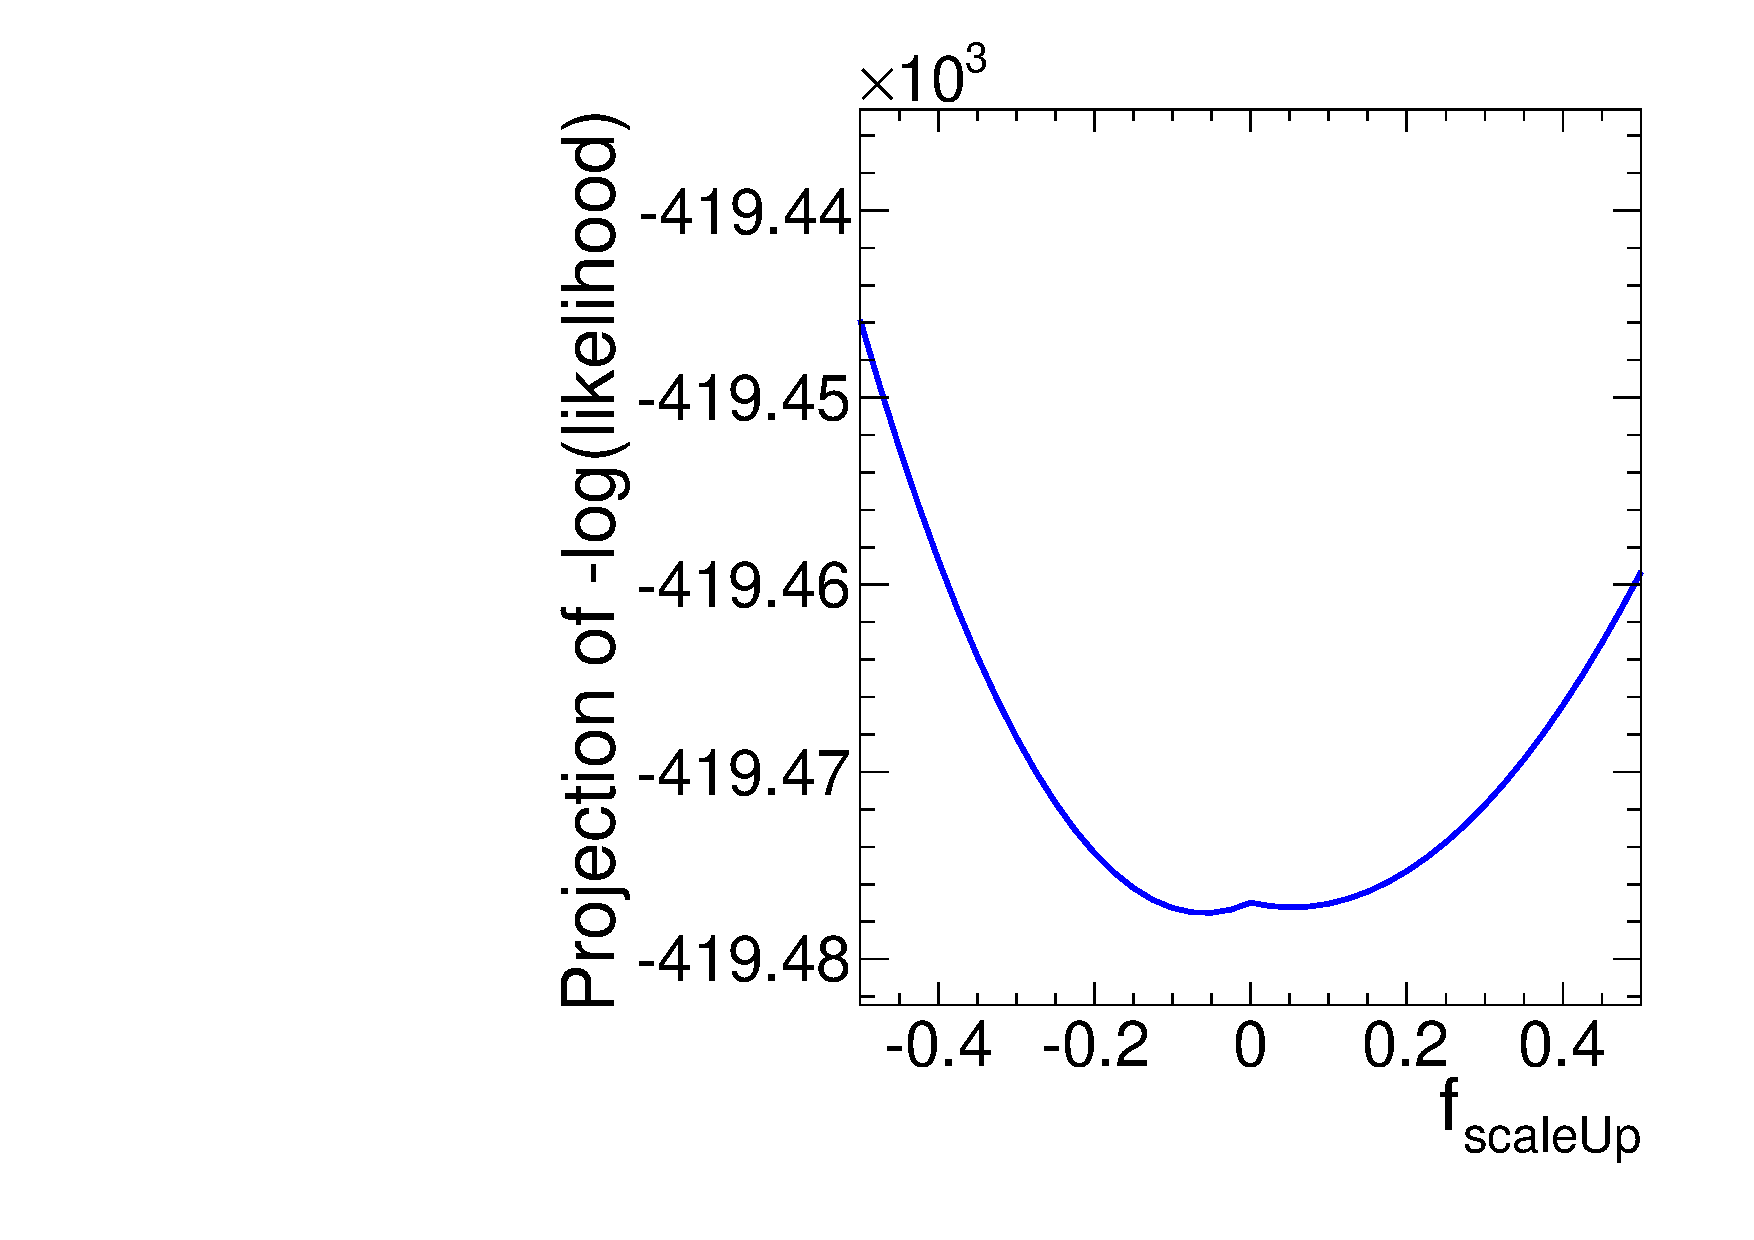
\includegraphics[width=0.48\textwidth]{figs/DibosonNLLfSU.pdf}
    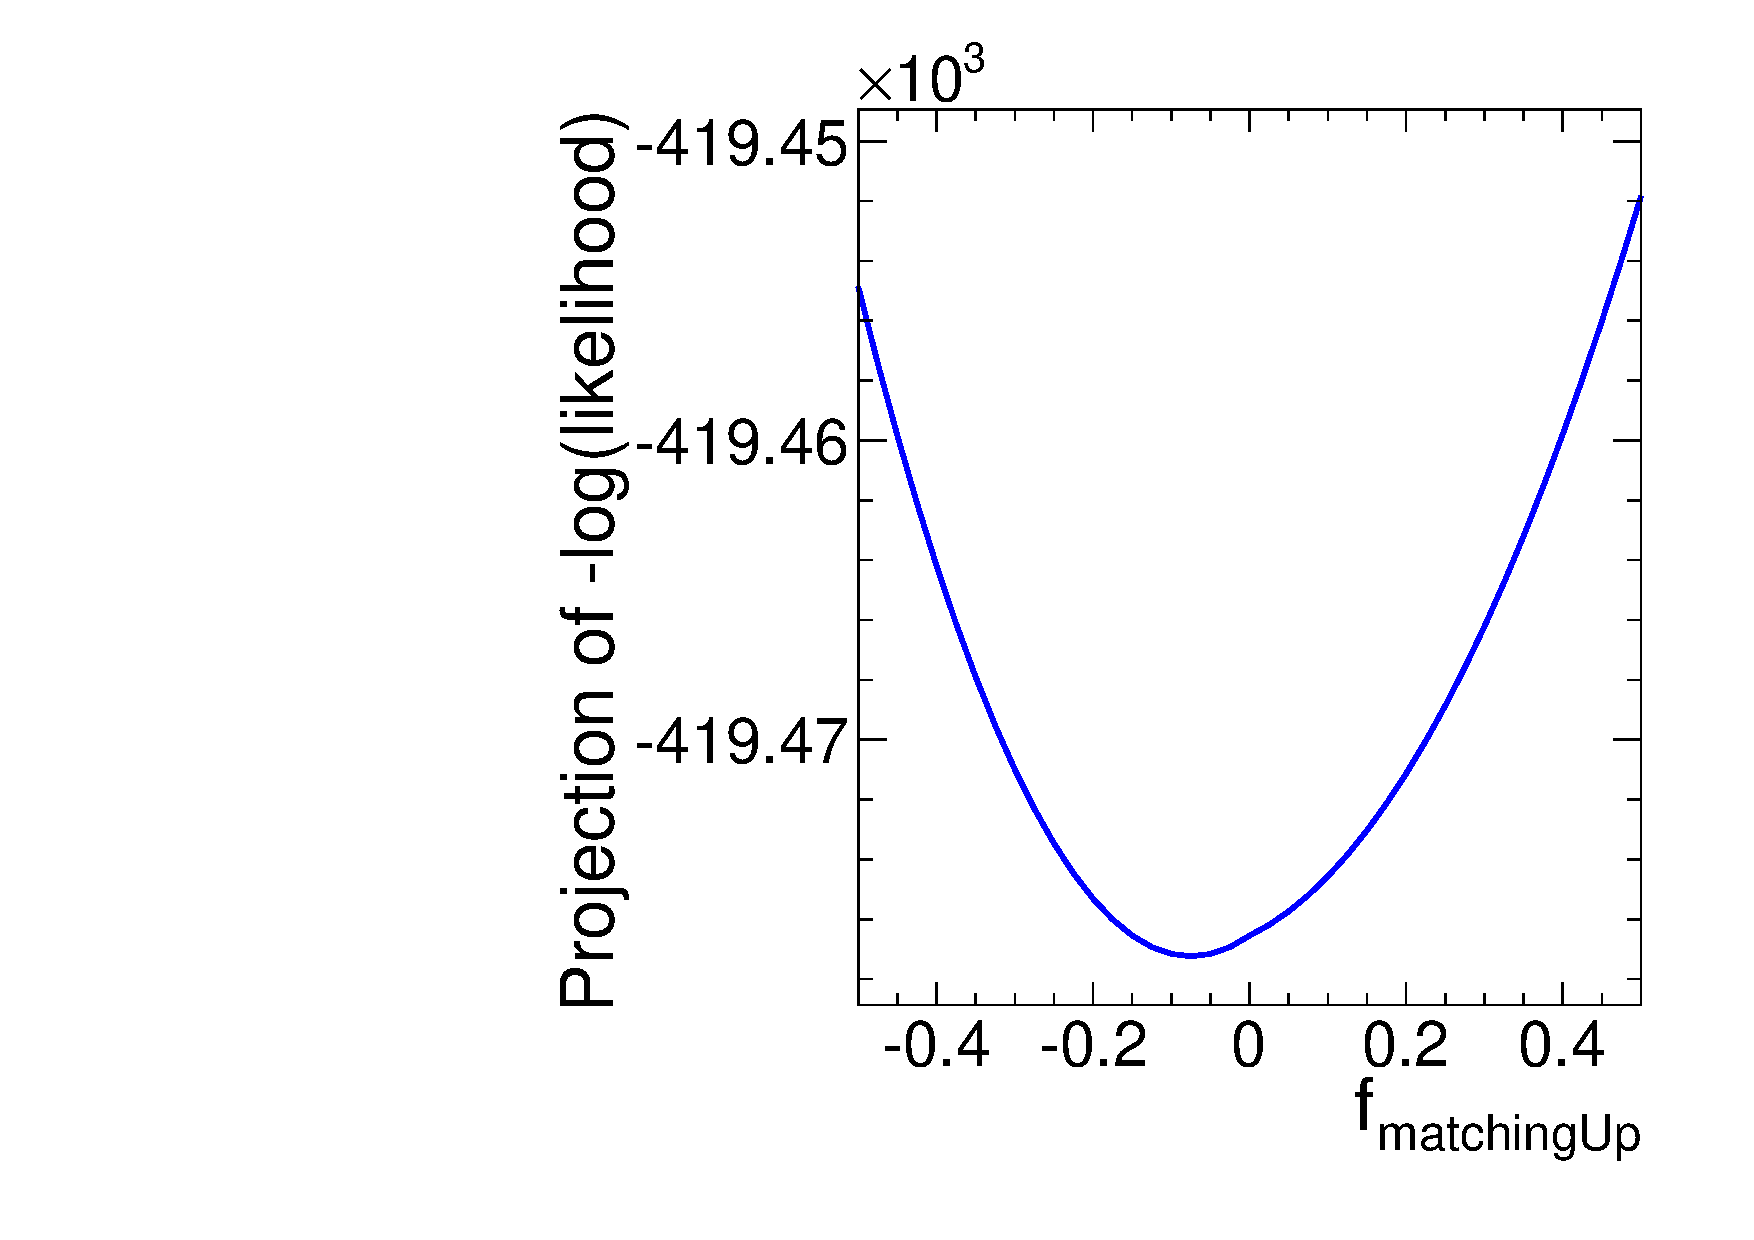
\includegraphics[width=0.48\textwidth]{figs/DibosonNLLfMU.pdf}
    \caption{The scan of the negative log likelihood for the 
factrization/renormalization and ME-PS matching scales. They have the 
usual parabolic distribution with minimum near 0. The minimum values 
correspond to the ones obtained in our nominal fit and listed in 
Table~\ref{tab:wjetsscale}. }
    \label{fig:q2NLLscan}}
\end{figure}
%%%%%%%%%%%%



%%%%%%%%%%%%%%%%%%%%%%%%%%%%%%%%%%%%%%%%%%%%
\subsection{Jet Energy Scale}
\label{sec:topw}
A dedicated analysis of 2010 data by the JetMET group showed that the jet energy
uncertainty for a generic particle-flow jet is within 3\% and the jet resolution
(JER) uncertainty is within 10\%.  For more details, see
Refs.~\cite{jetsyst,jetsyst2}.  The systematic uncertainties in the
JES and JER can affect our signal acceptance and the $m_{jj}$ distribution.
Figure~\ref{fig:ECComparison} shows a comparison of W+jets shape 
obtained using default jet energy scale with those obtained by using 
$\pm 1\sigma$ variation in the default scale.
In the present analysis, we performed several studies to cross check 
and constrain the JES/JER uncertainties. Two such studies are described 
below. We determine that the average uncertainty in the JES for the 
jet kinematics relevant to the present analysis is at the level below 1\% 
and uncertainty in JER is at the level of 10\%. These are in agreement 
with Refs.~\cite{jetsyst,jetsyst2} for jets of $p_T > 35$~\gev and 
$|\eta|<2.4$. The effect of propagating these uncertainties to the 
signal acceptance and diboson yields is minuscule. 
%%%%%%%%%%%%
%%%%%%%%%%%%
\begin{figure}[h!] {\centering
    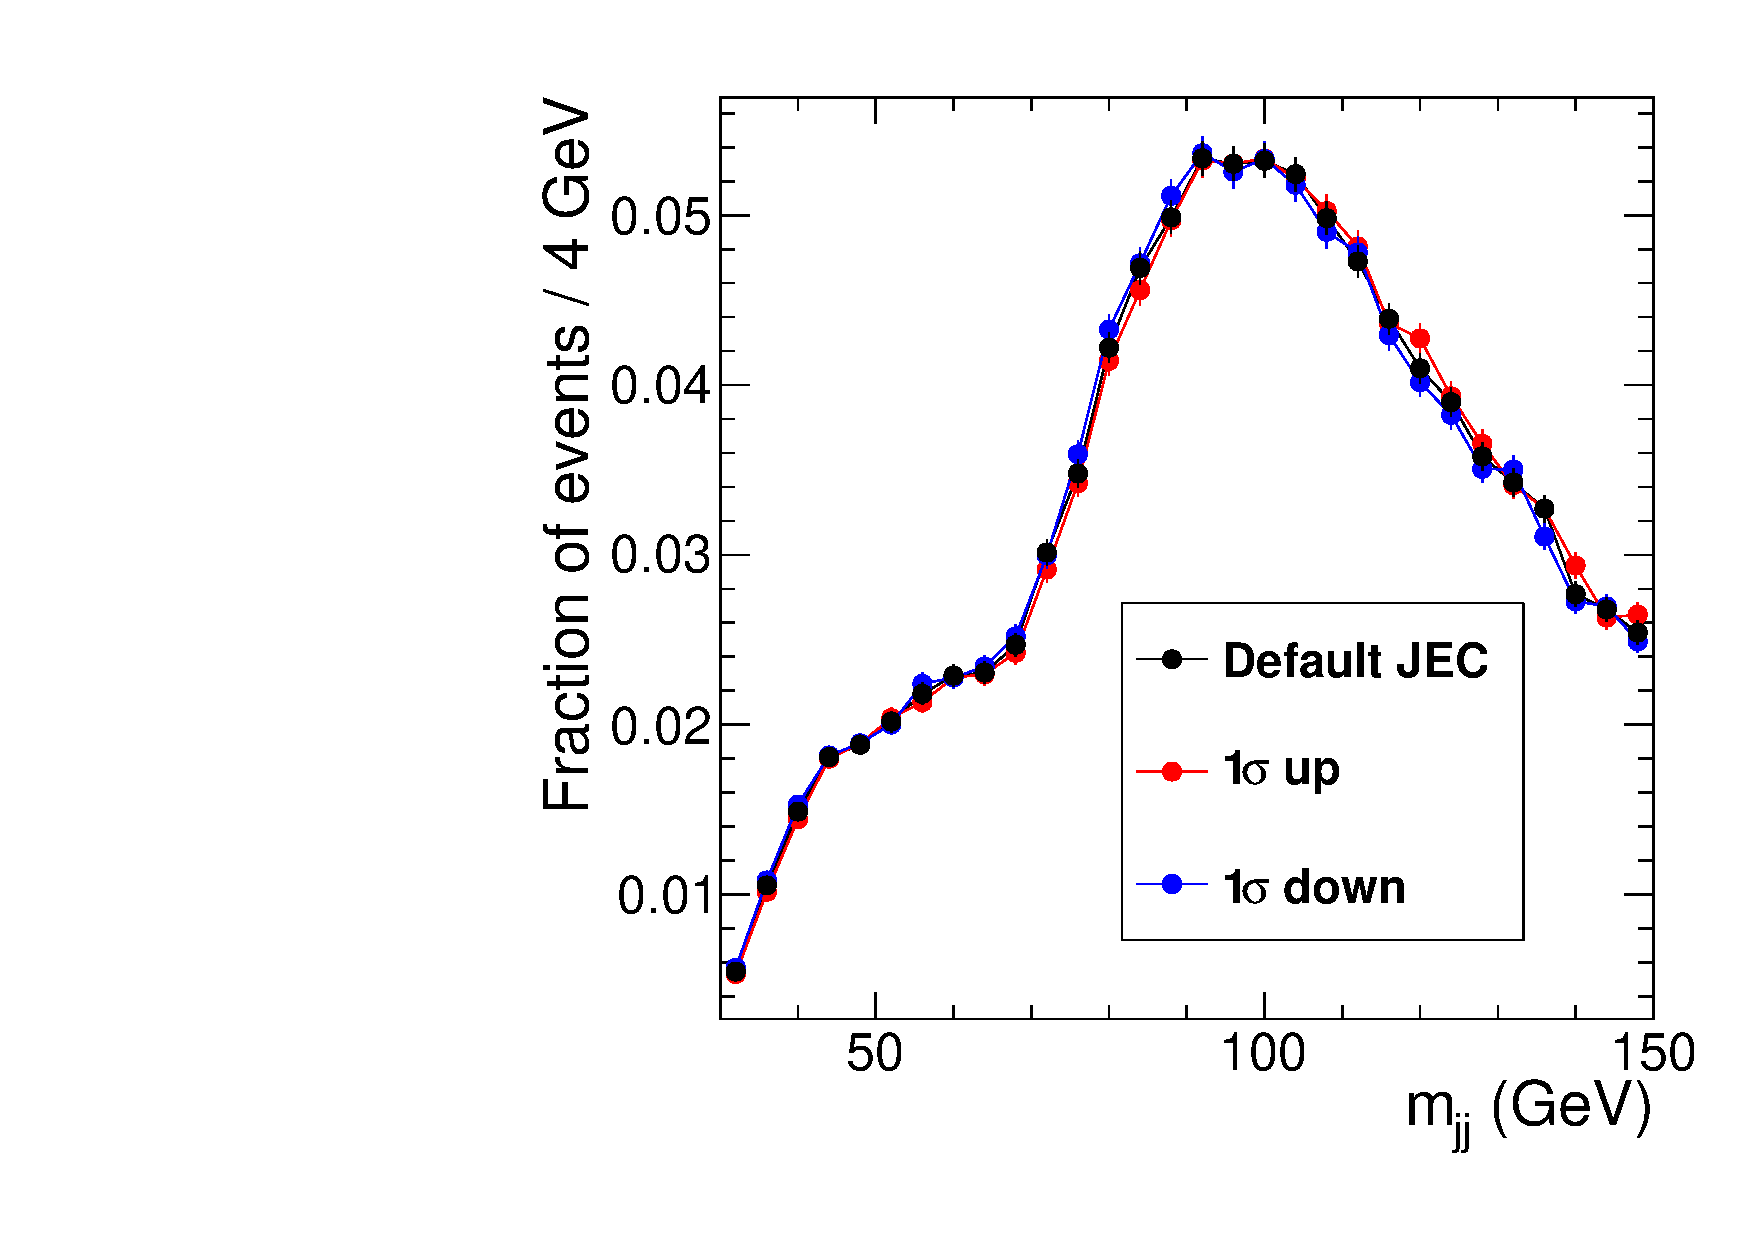
\includegraphics[width=0.5\textwidth]{figs/JECComparison.pdf}
    \caption{Comparison of W+jets shape using default JES and 
    using $\pm 1\sigma$ variation in JES. The selection used here 
    is the same as used for muon no b-tag data.}
    \label{fig:ECComparison}}
\end{figure}
%%%%%%%%%%%%
%%%%%%%%%%%%
%%%%%%%%%%%%
\subsubsection{Scan of jet energy scale}
In this study we scan the JES from -5\% to +5\% and repeat the fit. 
We performed  this test in a subset of the muon data. 
The $\chi^2$ of the fit is plotted in
Figure~\ref{fig:JESScanchi2} as a function of the JES shift. 

The minimum in $\chi^2$ is consistent
with the value obtained from hadronic W candidates in top
quark events (described below) and the fit has a stable, well defined minimum. 
Note that the above study serves a crosscheck.
%%%%%%%%%%%%
\begin{figure}[h!] {\centering
    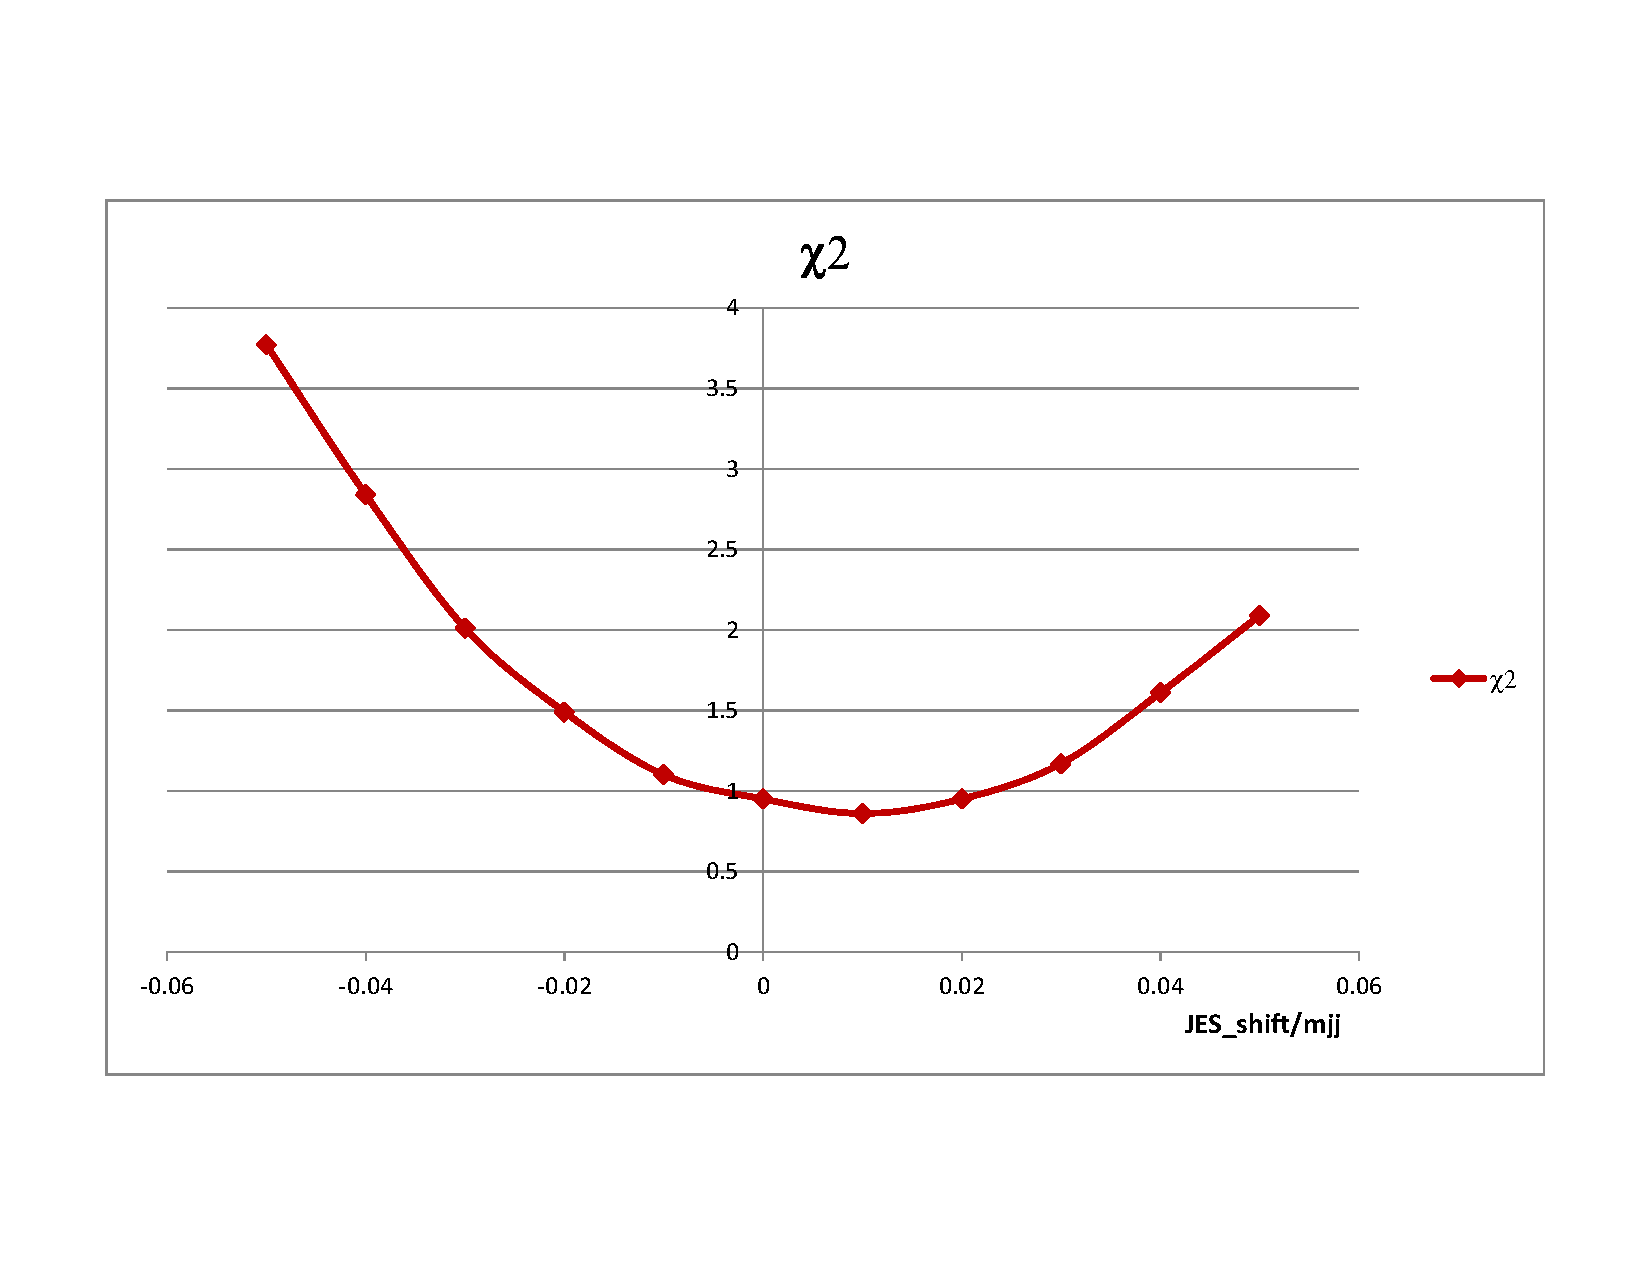
\includegraphics[width=0.5\textwidth]{figs/JES_scan.pdf}
    \caption{$\chi^2$ of the fit vs JES shift for muon no b-tag data.}
    \label{fig:JESScanchi2}}
\end{figure}
%%%%%%%%%%%%
\subsubsection{JES/ JER from the hadronic W in top quark events}
At LHC the top pair production rate is fairly large ($\sigma_{\ttbar}
= 163$~pb) -- almost four times larger than the diboson production
rate.  According to the Standard Model, the top quark decays into $W$
boson and $b$ quark with branching fraction of about 100\%.  If we
select events in which one $W$ boson decays leptonically
(\textit{i.e.}, $W\to e\nu, \mu\nu$) and the other $W$ boson decays
into quark pairs thus leading to a semileptonic final state, then the
signal purity is very high.  The final state consists of a high energy
lepton, large missing $E_T$, and four jets of which two are
$b$-tagged. The hadronic W candidates are formed from two anti-btagged
jets.  The invariant mass of the hadronic W candidates in the muon,
electron, and combined channels are shown in
Figs.~\ref{fig:topw:mu},~\ref{fig:topw:el}, and
\ref{fig:topw:muel}, respectively. 
The $W$ mass resolution is dominated by the resolution of the 
jet energy measurement.
When we propagate the difference in the JES to our
templates they make a negligible difference.
%%%%%%%%%%%%%%%%%%%%%
%%%%%%%%%%%%%%%%%%%%%
\begin{figure}[htb] 
  {\centering
    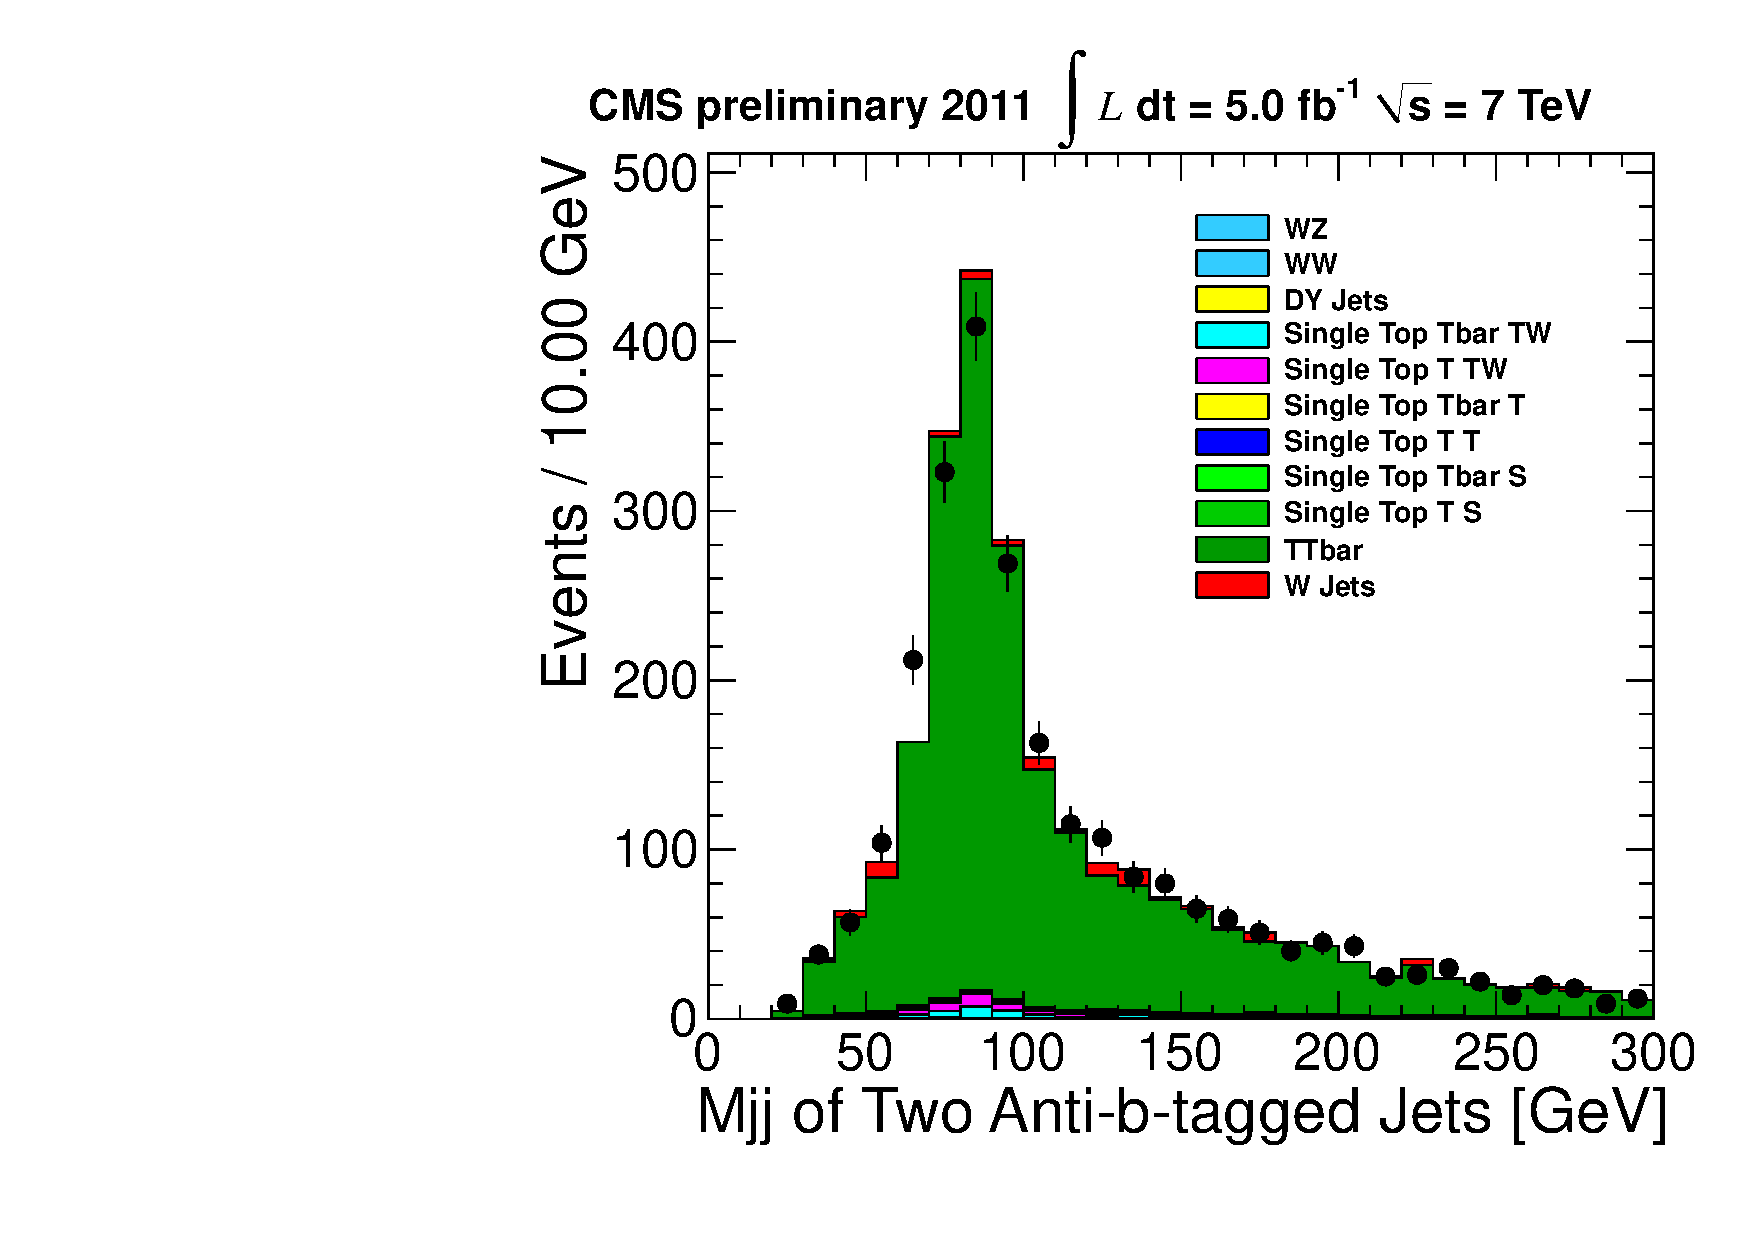
\includegraphics[width=0.49\textwidth]{figs/topwjes/top_overlap_mu.pdf}
    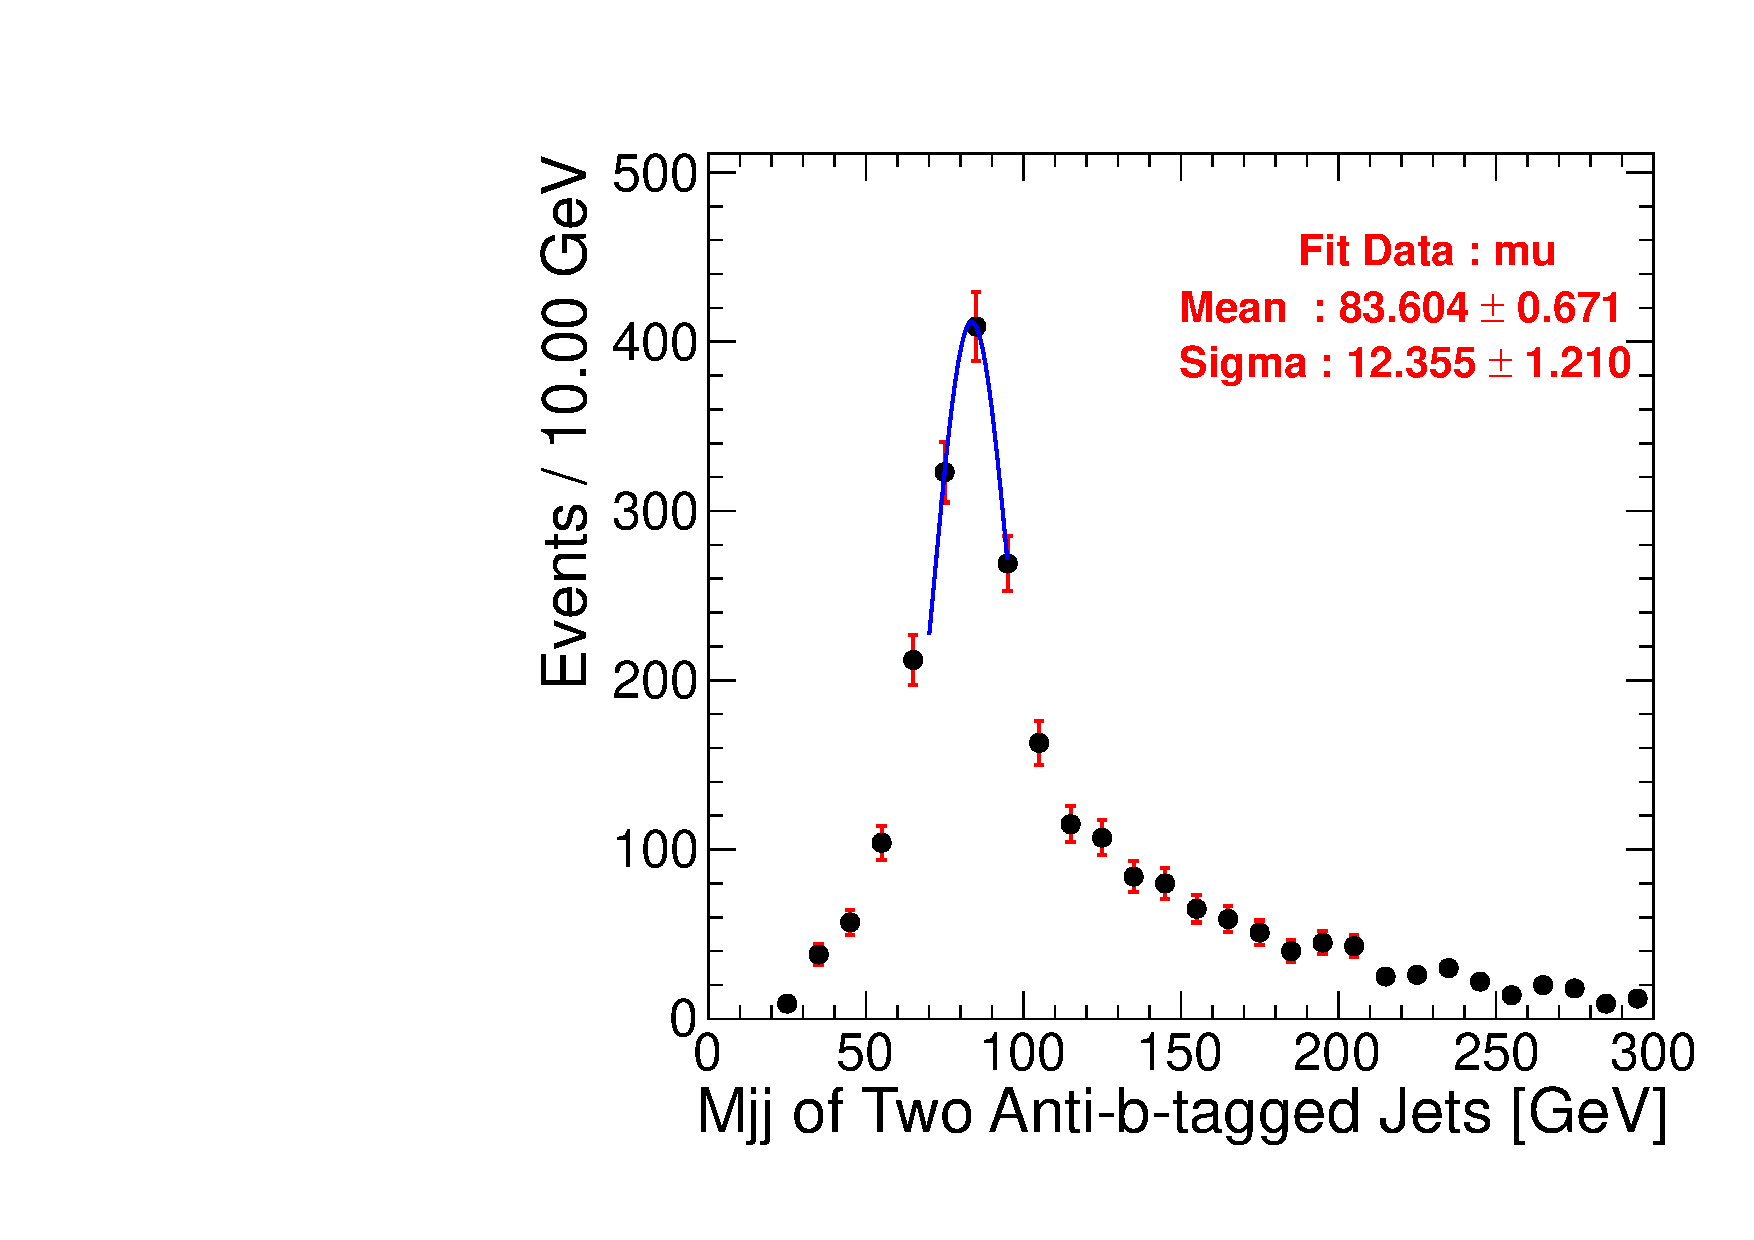
\includegraphics[width=0.49\textwidth]{figs/topwjes/top_data_fit_mu.pdf}
    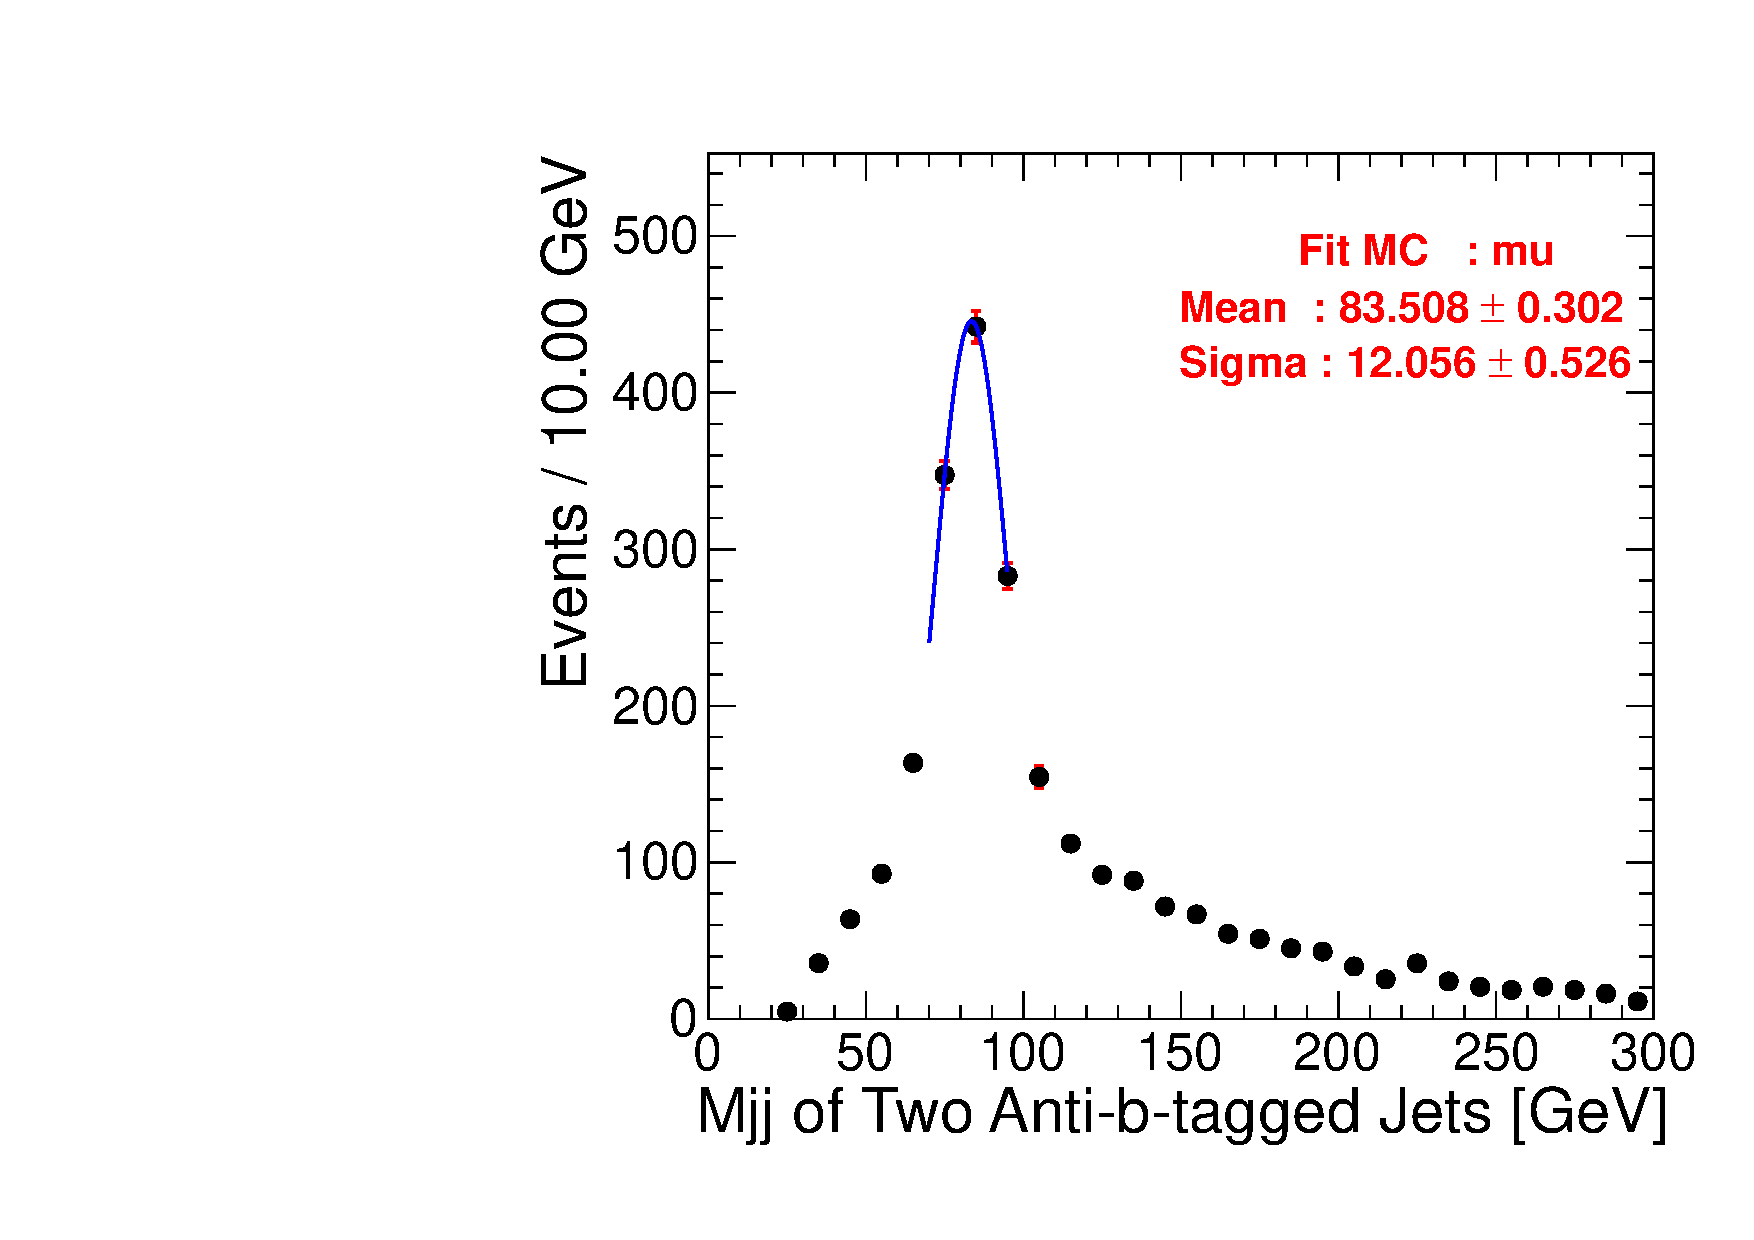
\includegraphics[width=0.49\textwidth]{figs/topwjes/top_mc_fit_mu.pdf}
    \caption{The invariant mass distribution of the hadronic 
      W candidates in the muon semileptonic top sample. The error bars 
      are statistical only.  
      The upper plot shows good agreement between the data and MC, and 
      can be compared to Figure~3a in TOP-11-015 (CERN record/1427762).
      We fit the distribution with a Gaussian and extract the peak
      location for the data (left) and MC (right).}
    \label{fig:topw:mu}}
\end{figure}
%%%%%%%%%%%%%%
\begin{figure}[htb] 
  {\centering
    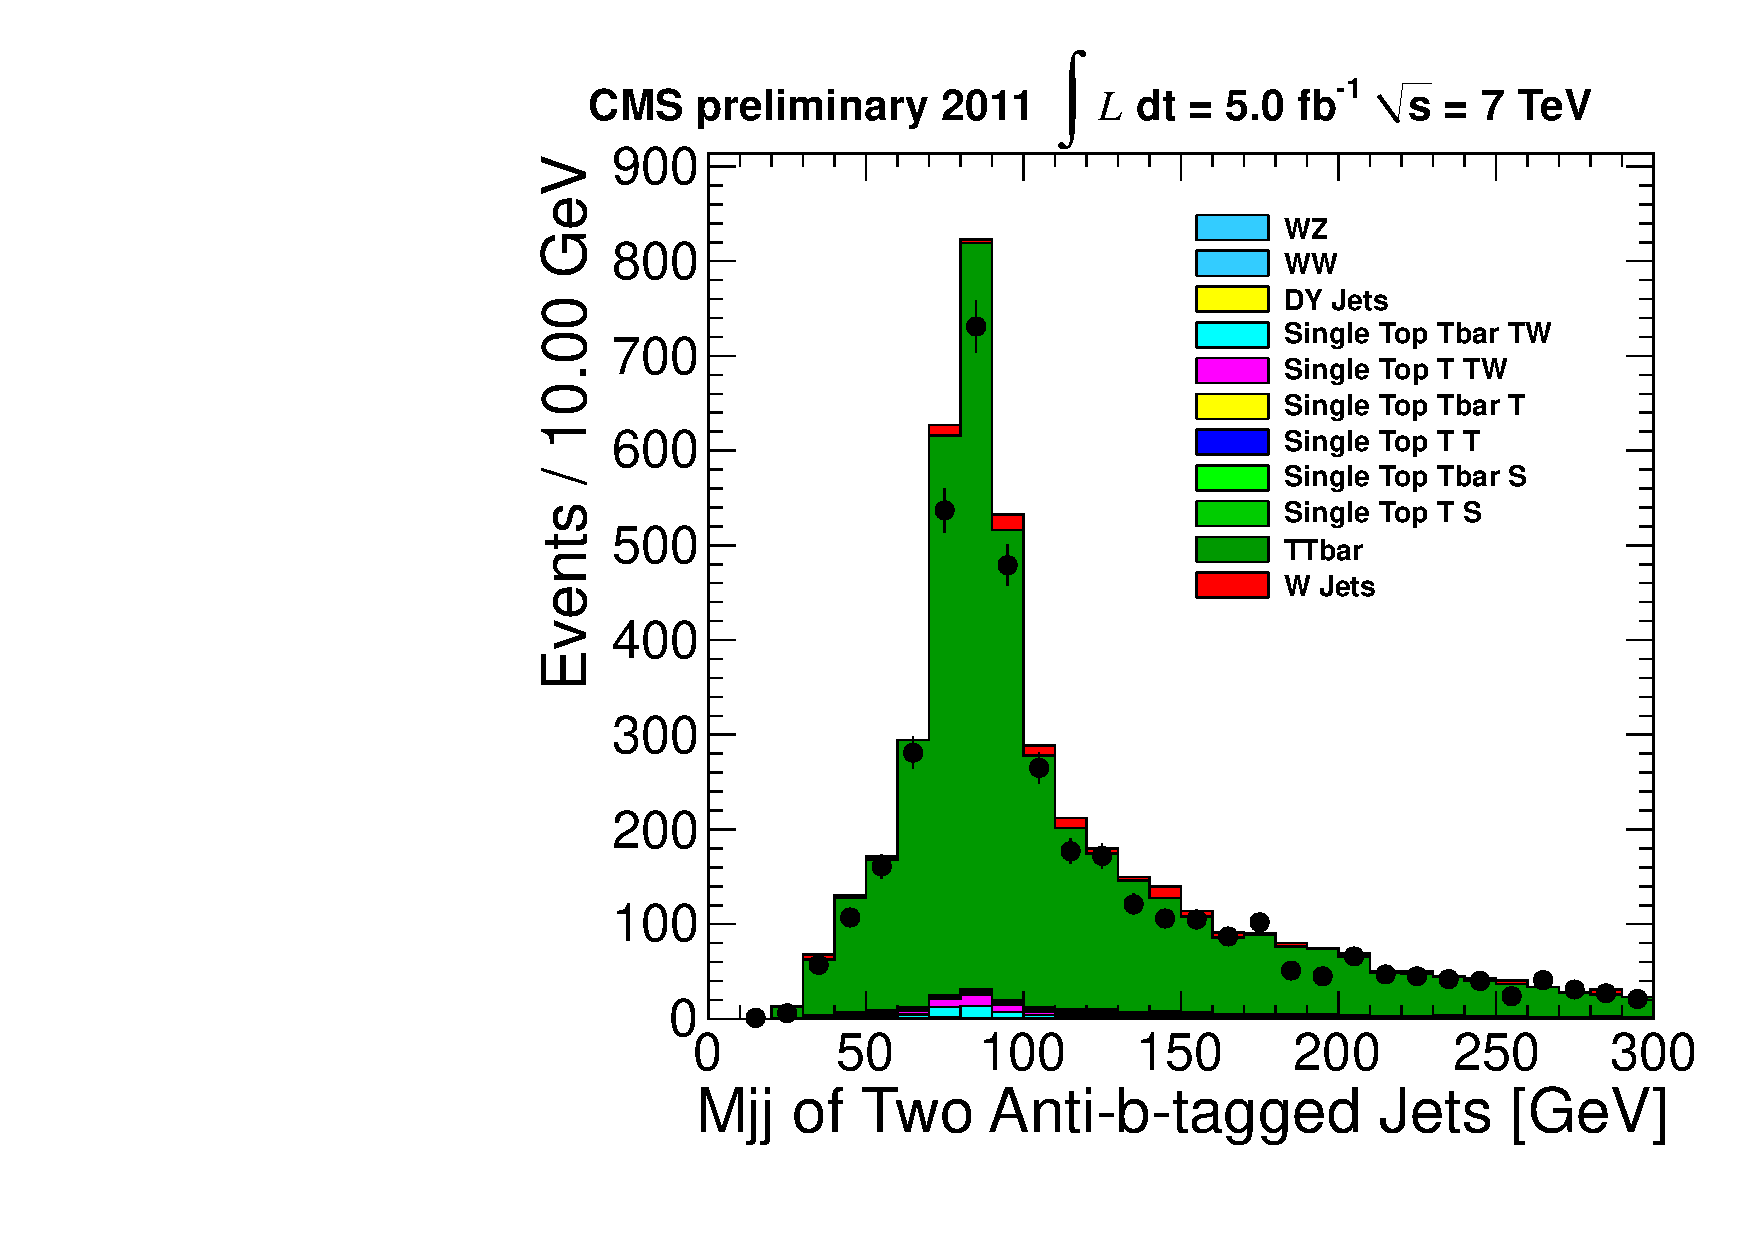
\includegraphics[width=0.49\textwidth]{figs/topwjes/top_overlap_el.pdf}
    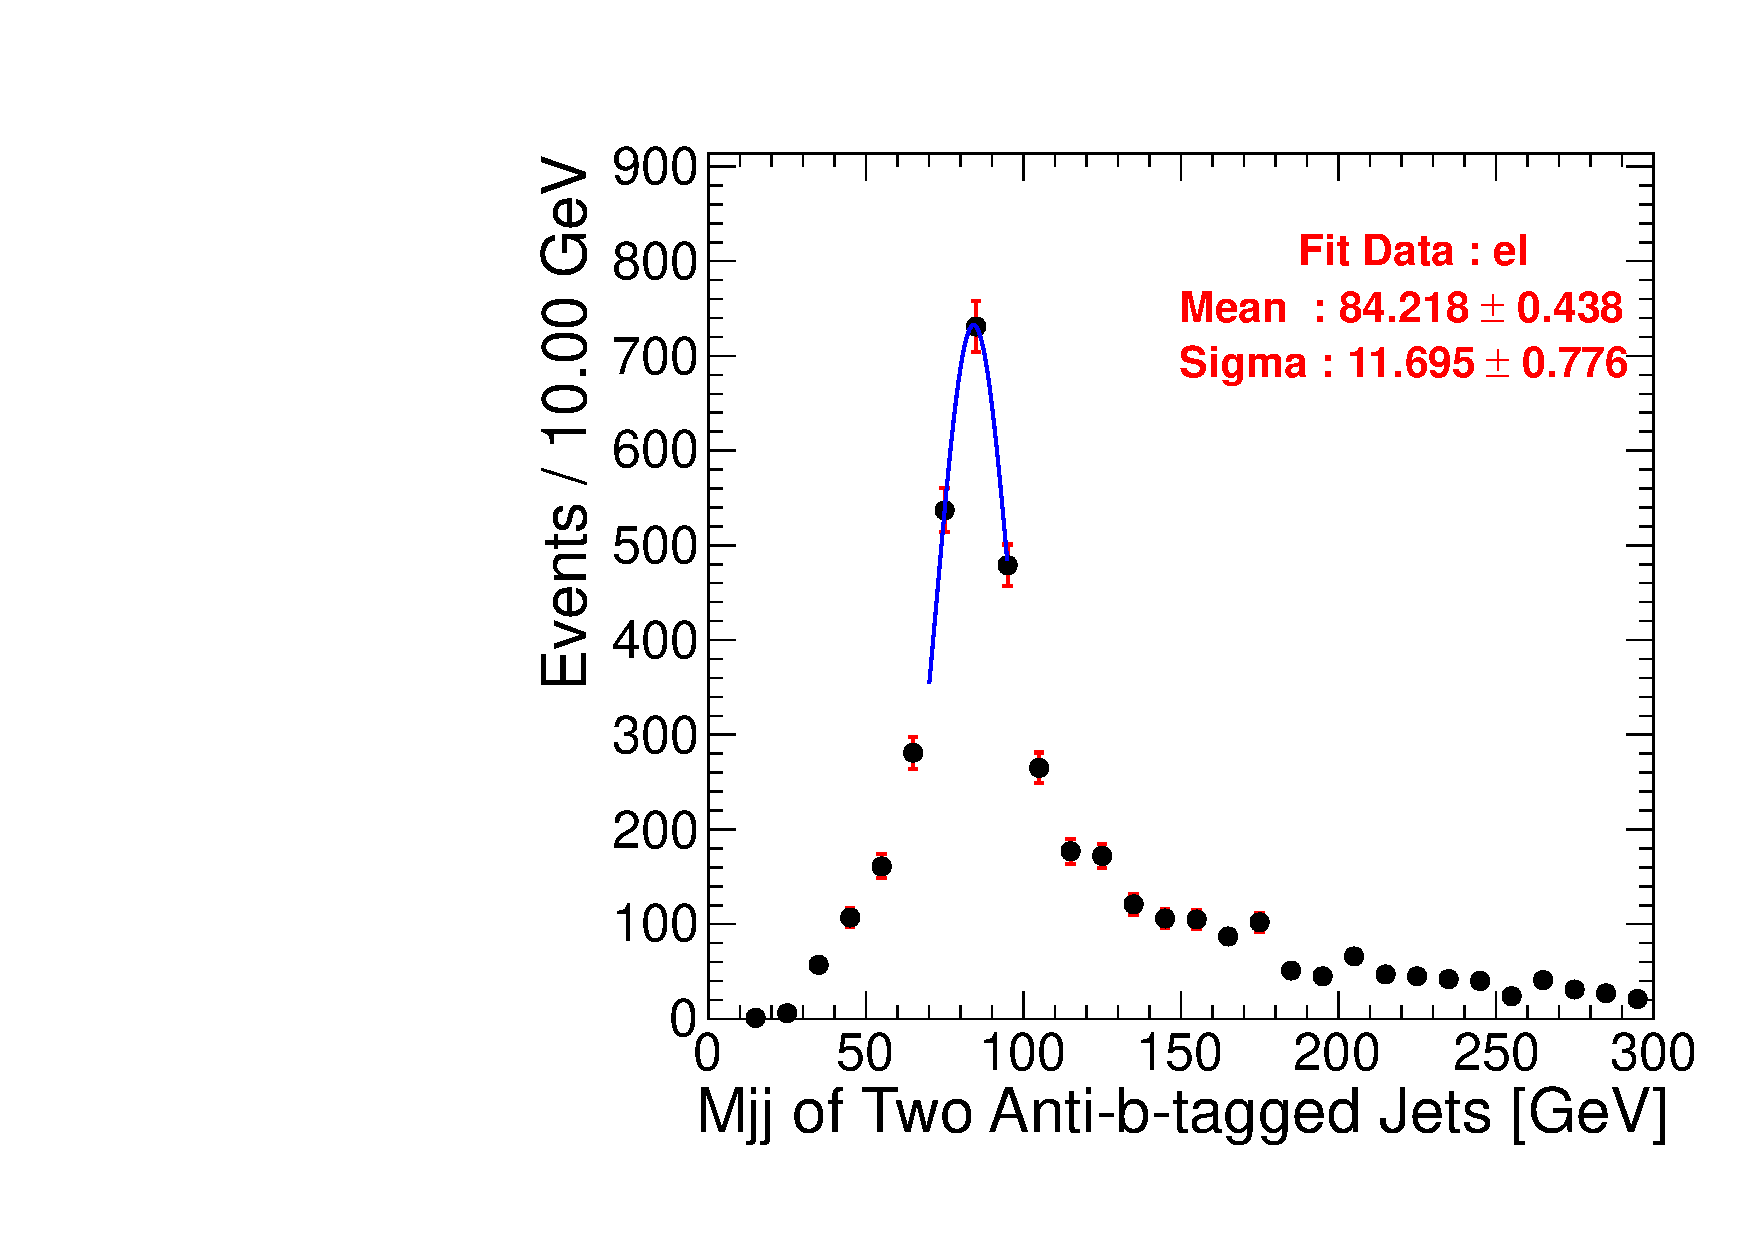
\includegraphics[width=0.49\textwidth]{figs/topwjes/top_data_fit_el.pdf}
    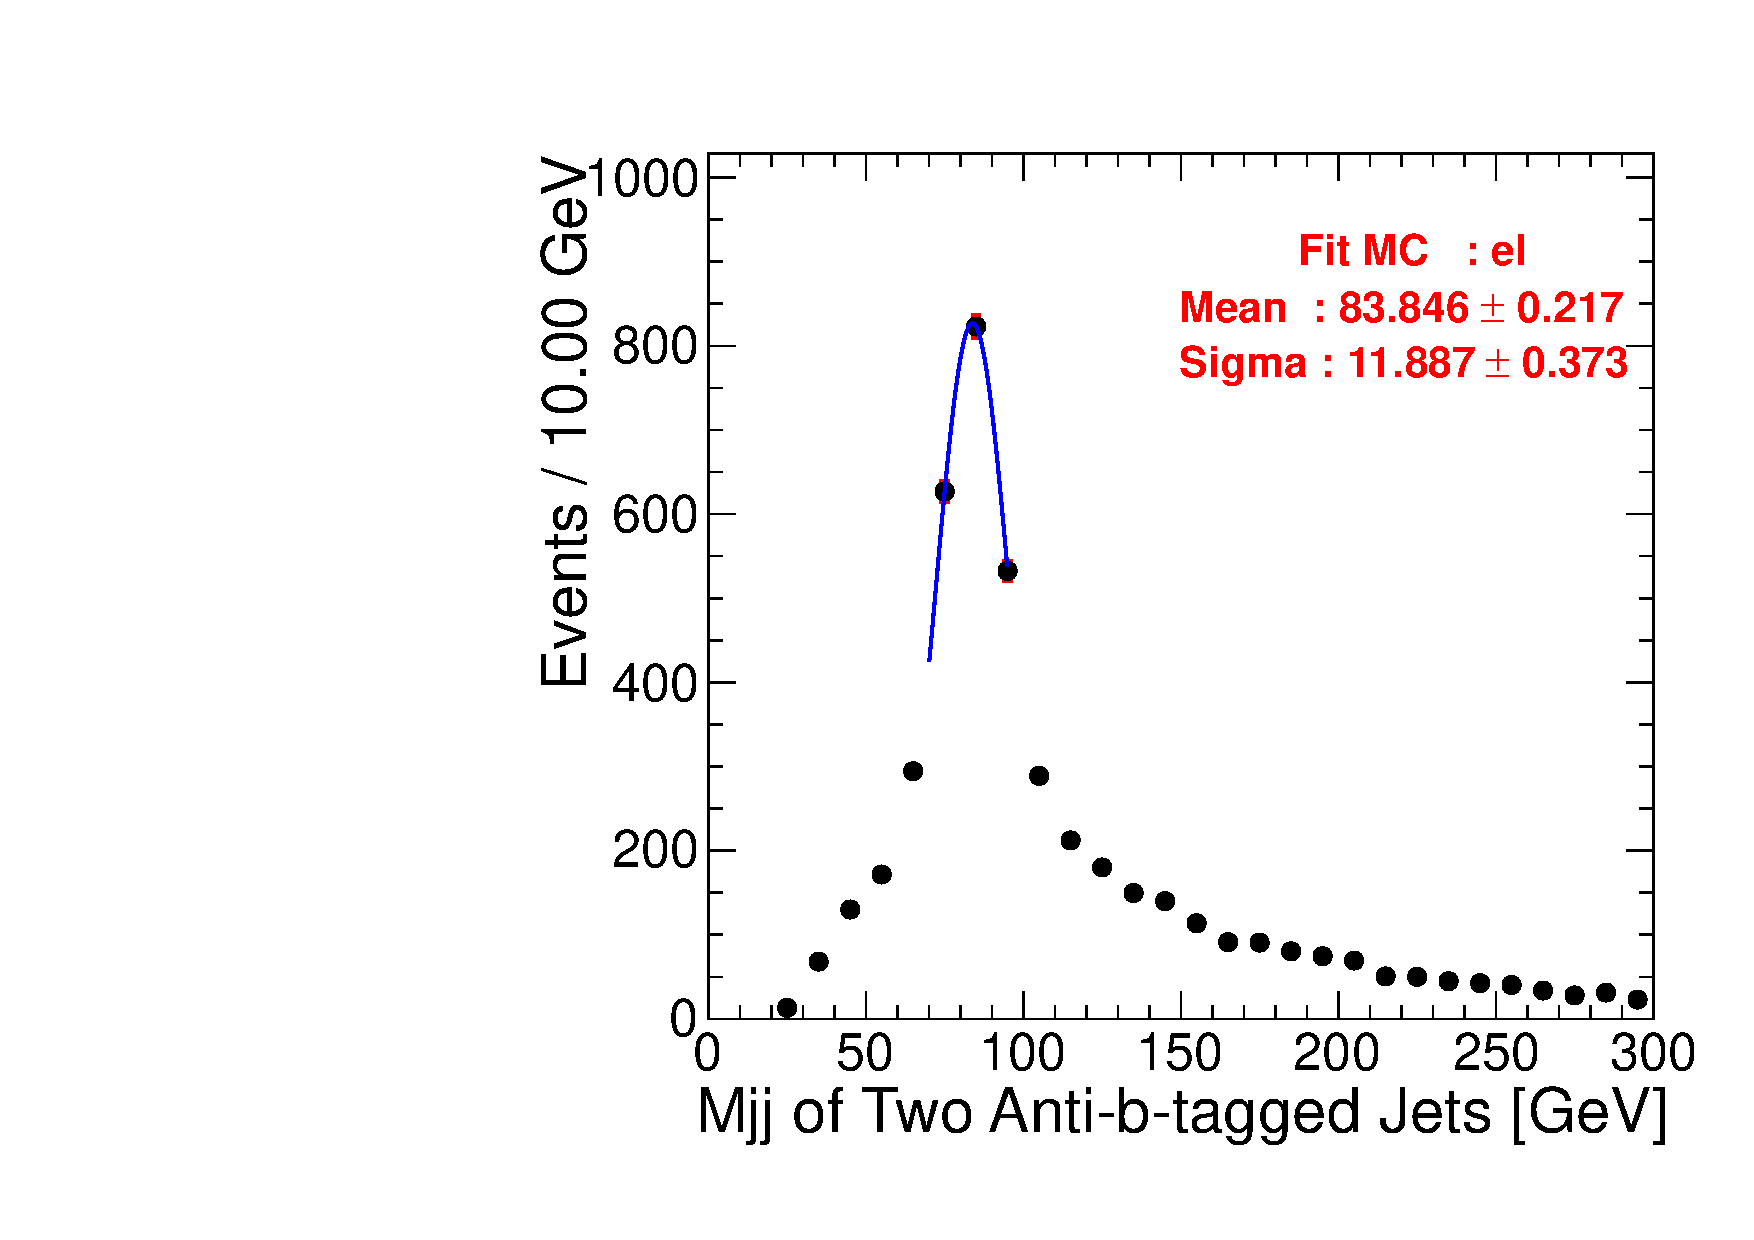
\includegraphics[width=0.49\textwidth]{figs/topwjes/top_mc_fit_el.pdf}
    \caption{The invariant mass distribution of the hadronic 
      W candidates in the electron semileptonic top sample. The error bars 
      are statistical only.  
      The upper plot shows good agreement between the data and MC, and 
      can be compared to Figure~3a in TOP-11-015 (CERN record/1427762). 
      We fit the distribution with a Gaussian and extract the peak
      location for the data (left) and MC (right).}
    \label{fig:topw:el}}
\end{figure}
%%%%%%%%%%%%%
\begin{figure}[htb] 
  {\centering
    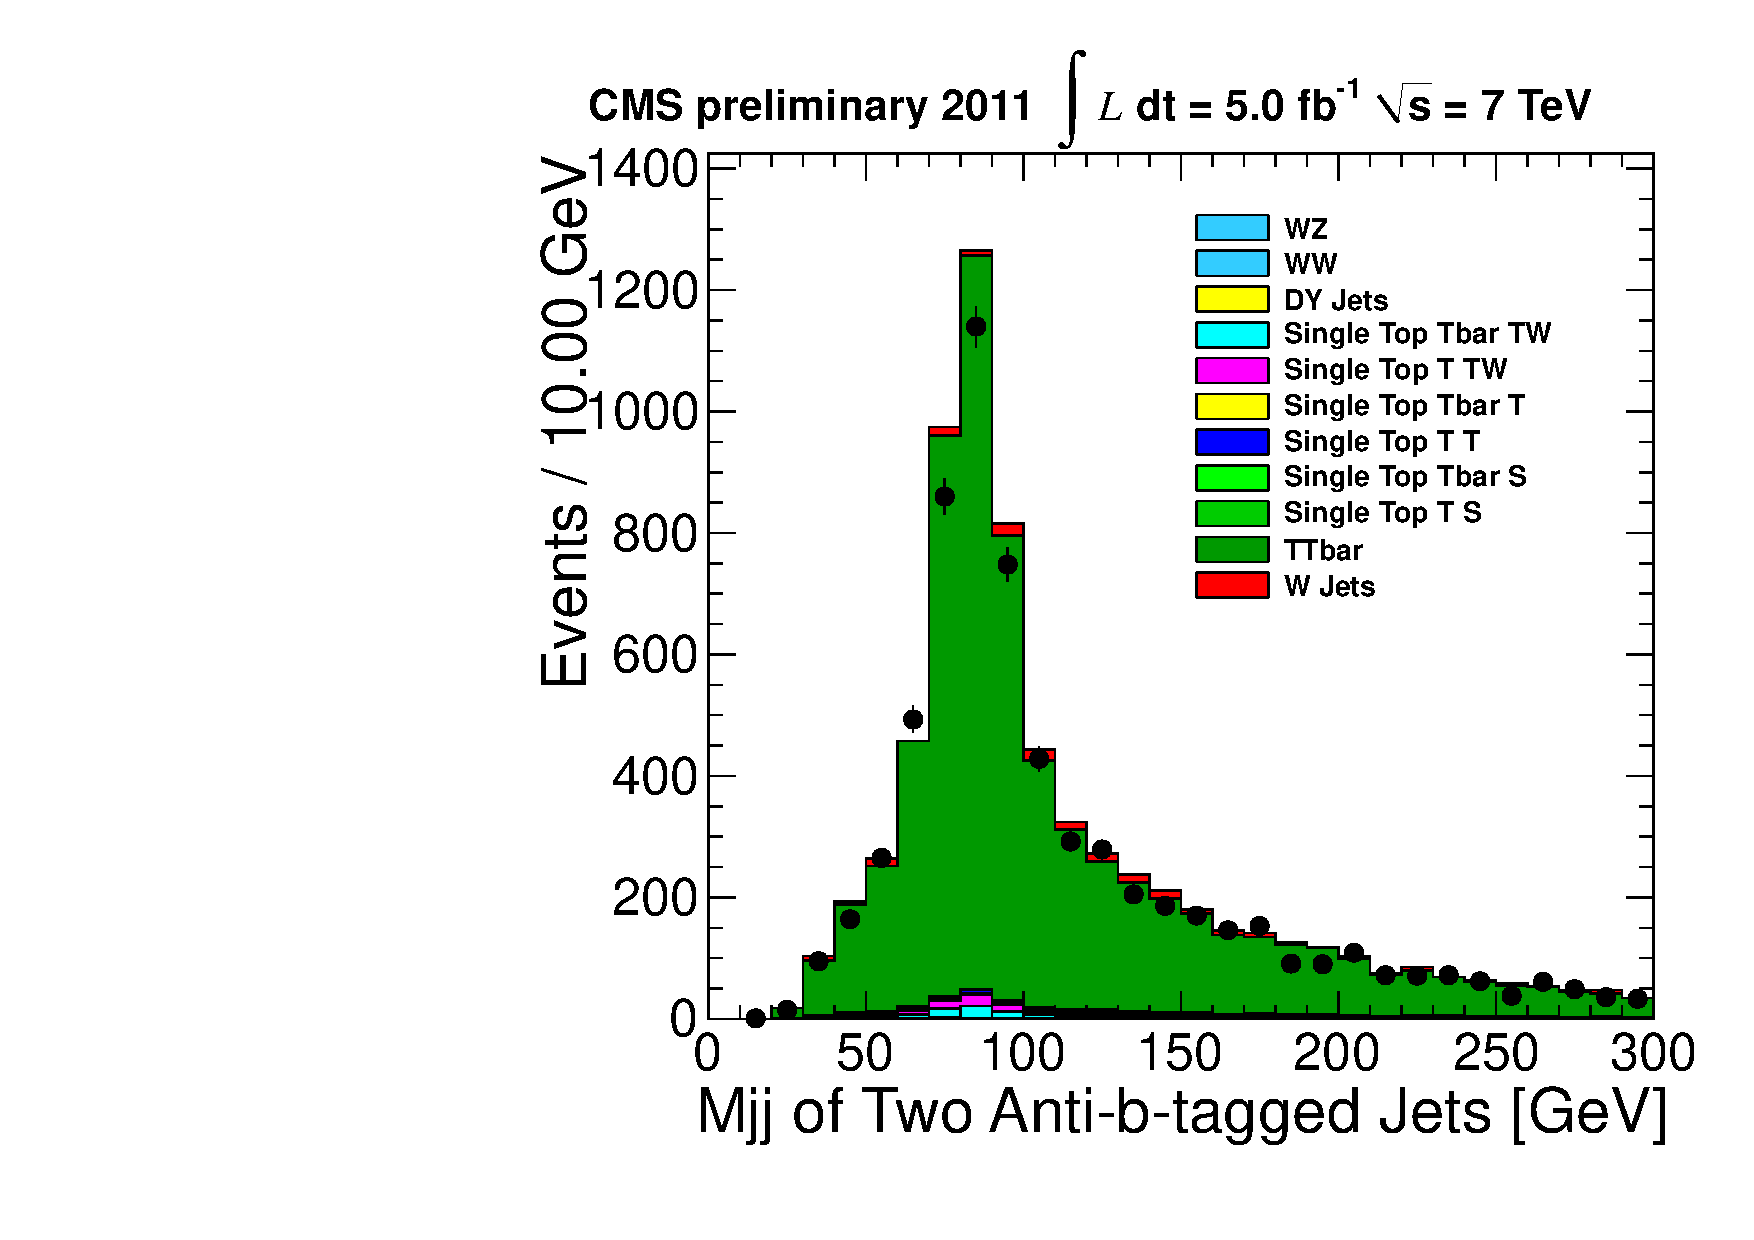
\includegraphics[width=0.49\textwidth]{figs/topwjes/top_overlap_muel.pdf}
    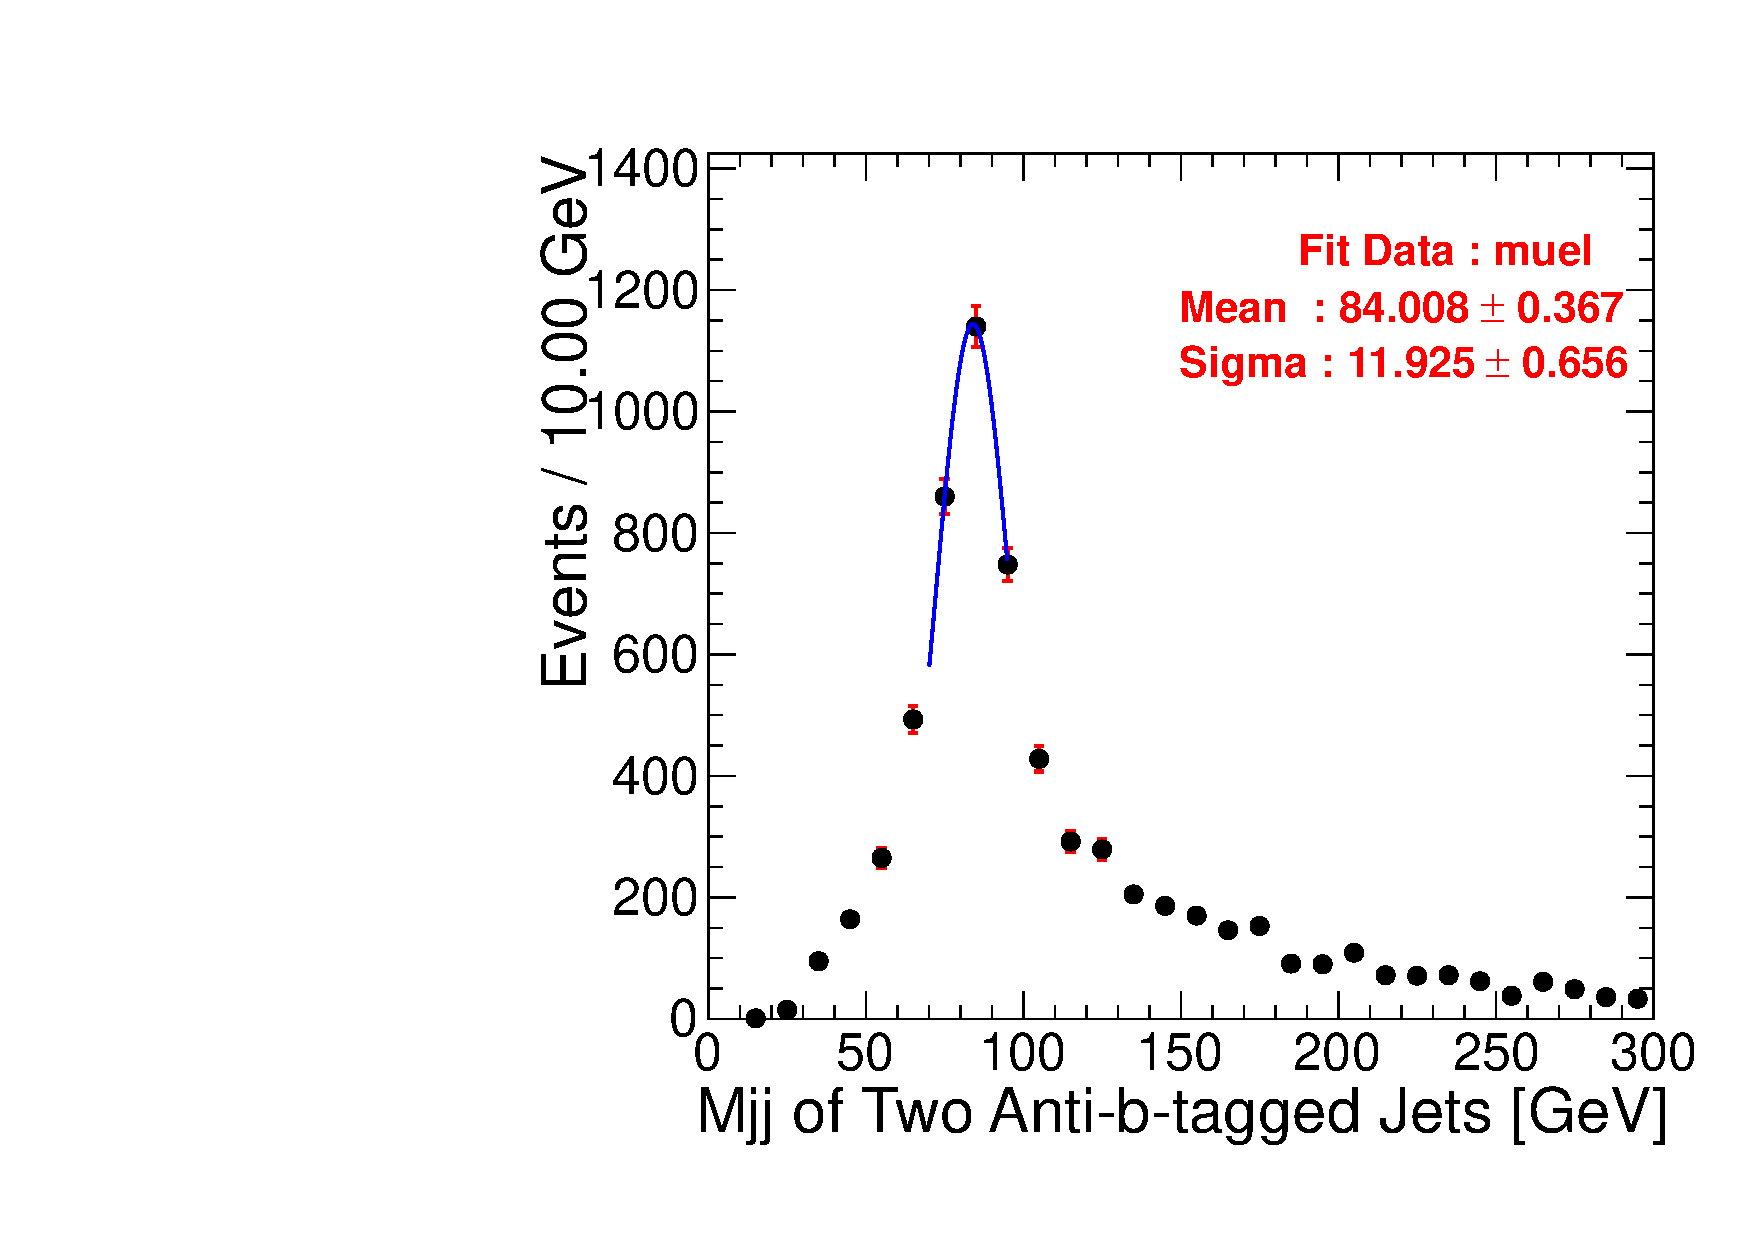
\includegraphics[width=0.49\textwidth]{figs/topwjes/top_data_fit_muel.pdf}
    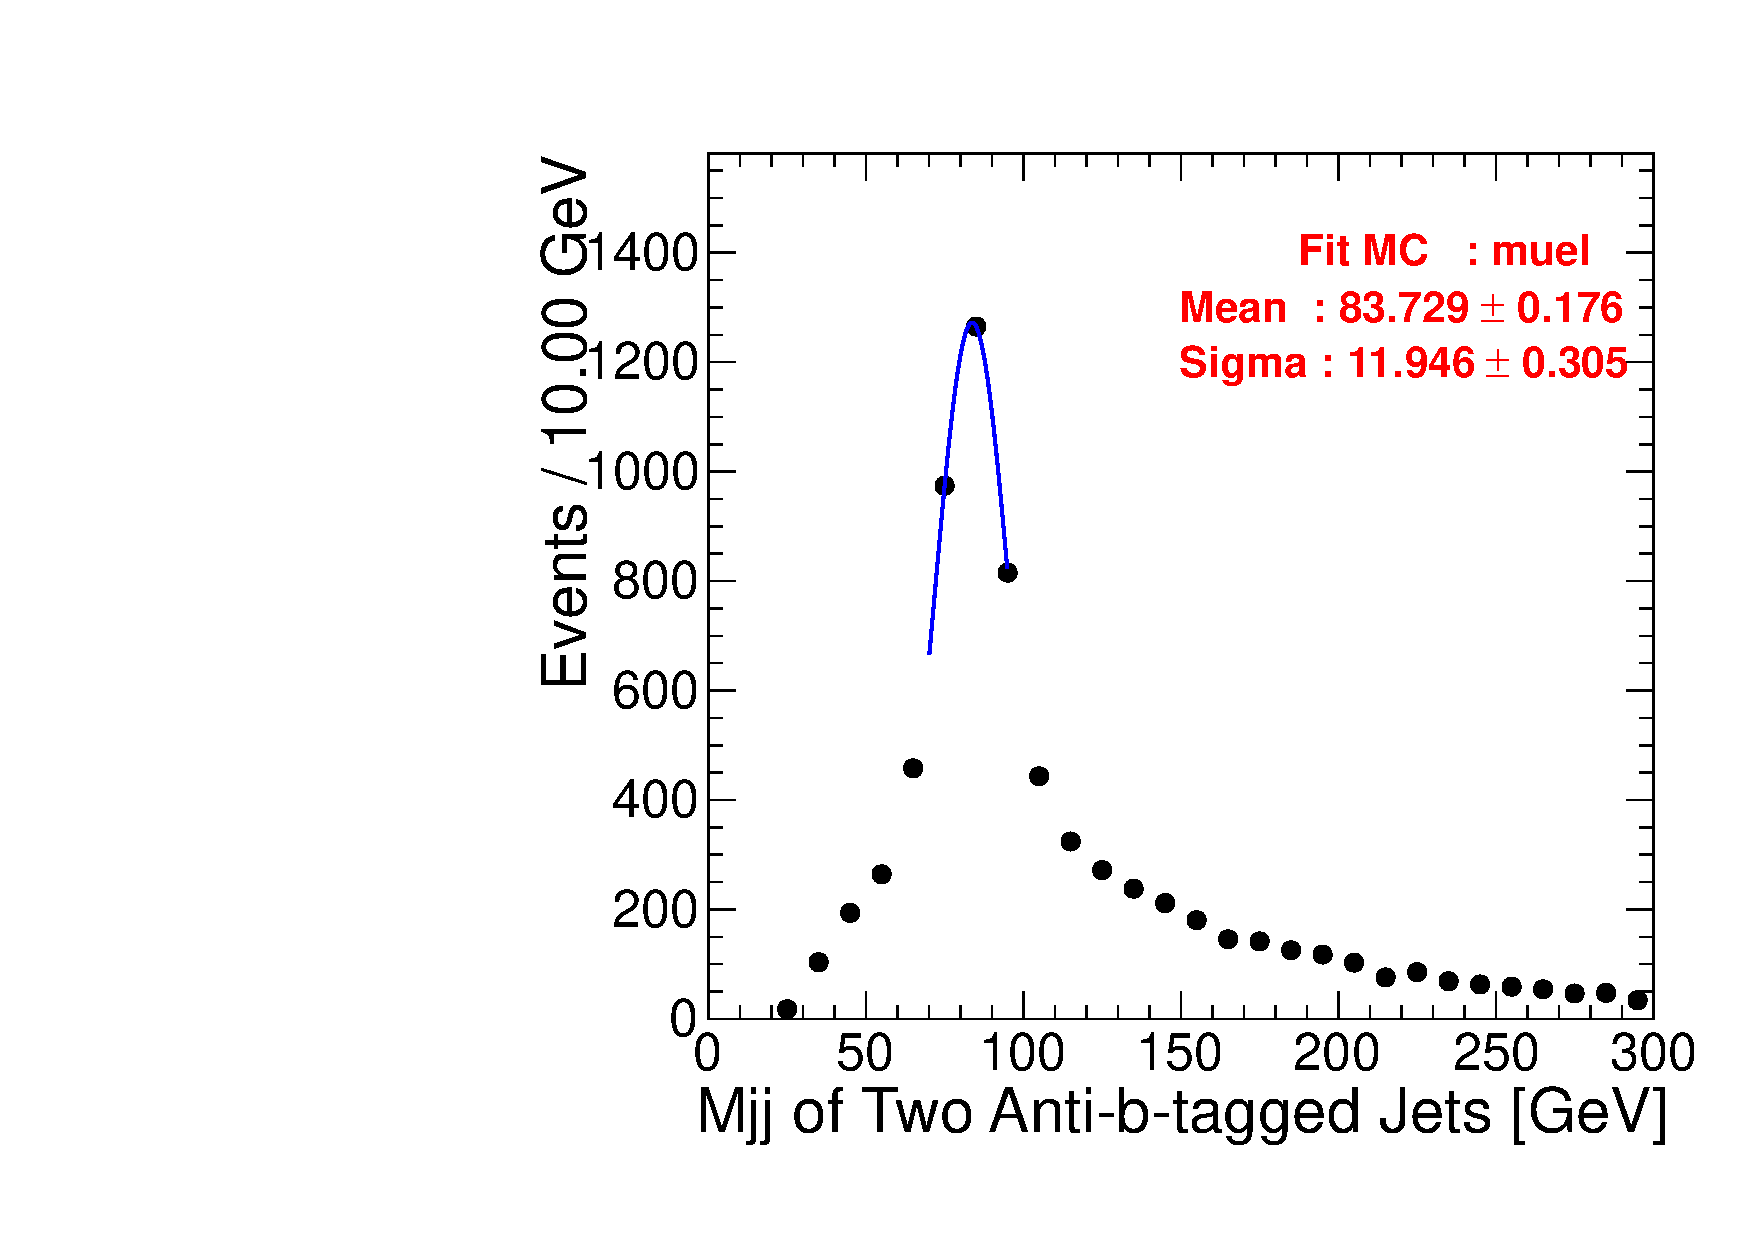
\includegraphics[width=0.49\textwidth]{figs/topwjes/top_mc_fit_muel.pdf}
    \caption{The invariant mass distribution of the hadronic 
      W candidates in the semileptonic top sample (electron and 
      muon combined). The error bars 
      are statistical only.  
      The upper plot shows good agreement between the data and MC, and 
      can be compared to Figure~3a in TOP-11-015 (CERN record/1427762). 
      We fit the distribution with a Gaussian and extract the peak
      location for the data (left) and MC (right).}
    \label{fig:topw:muel}}
\end{figure}
%%%%%%%%%%%%%%%%%%%%%%%%%%%%%%%%%%%%%%%%%%%%%%%%%%%%%%%%%%%%%%%%%%%%%%%%%%%
%--------------------------------------------------
\subsection{Lepton selection and trigger efficiency}
\label{sec:LeptonSelectionAndTriggerEfficiency}
%%The lepton trigger and selection is common among several CMS analyses and 
%%we benefit from common studies based on tag-and-probe techniques. 
%%
Systematic uncertainties in the trigger efficiencies in
Section~\ref{sec:trigger} are of the order of 1\%. Systematic
uncertainties in the lepton reconstruction and identification
efficiency scale factors are of the order of 2\%. These uncertainties
are accounted for in the final systematics that are input to the
cross-section uncertainty calculation.
%--------------------------------------------------
\subsection{MET uncertainty}
MET directly affects our signal acceptance. 
The uncertainty prescription is discussed in Ref.~\cite{met}.
%https://twiki.cern.ch/twiki/bin/viewauth/CMS/MissingETUncertaintyPrescription
In addition, the MET distribution in the data is $\simeq$3\% wider 
than the MC, and placing a hard MET$>30.0$ cut creates an uncertainty. 
We estimate it by smearing the MET for each event by a Gaussian with 
a $\sigma =0.03*$MET and observing how many events pass the cut. 
Specifically, (Events Passing After Smearing)/(Events Passing Before Smearing) 
=0.998 for both muons and electrons.
%%%%%%%%%%%%%%%%%%%%%%%%%%%%
\subsection{Cross-section of nuisance backgrounds}
The uncertainties in the cross sections of other backgrounds 
like $\ttbar$,  single top, QCD multi-jets, and Z+jets processes 
are already propagated by letting their normalization (i.e., yield) 
float in the fit within a constraint.

%%%%%%%%%%%%%%%%%%%%%%%%%%%%
\subsection{Theory uncertainty in acceptance}
We compute theory uncertainty in acceptance for muon ``no b-tag'' selection 
using MCFM: $\pt^{\text{jet}}>35$~GeV, $|\eta^{\text{jet}}|<2.4$, 
$\pt^{\text{lepton}}>325$~GeV, $|\eta^{\text{lepton}}|<2.1$, 
$\met > 30$~GeV, W $m_T > 30$~GeV, $\Delta{R}$ (lepton, jet) $>0.3$, 
no additional lepton. 
We use CTEQ6.6m as the default PDF and the quantity $\mu_0 = \sqrt{M_W^2 + p_{T, W}^2}$ as  
the default factorization/renormalization scale.
For systematic studies 
we vary the choices of PDF and the factorization/renormalization 
scale. The details are shown in Table~\ref{tab:theorysyst}. 
The overall theory 
uncertainty is below 3\%.
%%%%%%%%%%%%%%%%%%%%%%%%%%
 \begin{table}[h!]
   \begin{center}
   \begin{tabular}{l|c}
  \hline
  \hline
  Source of uncertainty & Relative variation in acceptance value \\
  \hline                                  
  PDF: CT10                             & $1.4\%$ \\
  PDF: CTEQ61M                          & $-0.7\%$ \\
  PDF: MSTW8NL                          & $0.4\%$ \\
  PDF: MSTW8NN                          & $0.1\%$ \\
  PDF: MSTW8LO                          & $-1.3\%$ \\
  Scale: $2~\mu_0$                      & $-0.01\%$ \\
  Scale: $0.5~\mu_0$                    & $0.8\%$ \\
  Scale: $\sqrt{M_W^2 + p_{T, jet1}^2}$ & $-0.3\%$ \\
  Scale: $H_T$                          & $0.1\%$ \\
  \hline
  \hline
   \end{tabular}
   \end{center}
   \caption{Theory uncertainty in acceptance. The central value for 
   acceptance $\times$ branching fraction is $(1.279 \pm 0.019) \times 10^{-2}$.} 
   \label{tab:theorysyst}
 \end{table}
%%%%%%%%%%%%%%%%%%%%%%%%%
%%%%%%%%%%%%%%%%%%%%%%%%%%%%
\subsection{Uncertainty in jet veto efficiency}
Since we use events with exactly two jets, we reject signal events 
which have extra jet(s) from ISR or FSR. Our acceptance computation 
takes this inefficiency into account. However, there is a 
systematic uncertainty associated with the modeling of 
ISR/FSR in our simulation. To estimate this systematics we 
compare the efficiency of our jet veto at generator-level 
(i.e., using ``GenJets'') in the Pythia WW, Pythia WZ, and 
privately produced MadGraph WW samples. All three simulations 
use LO matrix element calculation, parton showering from 
Pythia, and identical choices of factorization/renormalization
scales and PDFs. However, the soft gluon radiation probability 
is different in each sample.  
Table~\ref{tab:jetvetoeff} lists the jet-veto efficiency 
in each of the three samples. We take the maximum 
difference in efficiency as a systematic uncertainty.
This systematic is within 2\%.
%%%%%%%%%%%%%%%%%%%%%%%%%%
 \begin{table}[h!]
   \begin{center}
   \begin{tabular}{l|c}
  \hline
  \hline
  Sample & jet-veto efficiency \\
  \hline                                  
  WW Pythia                             & $88.72\%$ \\
  WZ Pythia                             & $87.48\%$ \\
  WW MadGraph                           & $89.57\%$ \\
  \hline
  \hline
   \end{tabular}
   \end{center}
   \caption{Jet-veto efficiency in various diboson simulations.} 
   \label{tab:jetvetoeff}
 \end{table}
%%%%%%%%%%%%%%%%%%%%%%%%%
%%%%%%%%%%%%%%%%%%%%%%%%%%%%
\subsection{Luminosity uncertainty}
The latest recommendation for the uncertainty on LHC luminosity is 2.2$\%$~\cite{lumiPAS}.
We propagate this uncertainty to the expected yield of the signal and from there to the
calculated cross-section.
%%%%%%%%%%%%%%%%%%%%%%%%%%%%
%%%%%%%%%%%%%%%%%%%%%%%%%
 \begin{table}[h!]
   \begin{center}
   \begin{tabular}{l|c}
  \hline
  \hline
  Source of uncertainty & Magnitude \\
  \hline                                  
  Luminosity                             & $2.2\%$ \\
  Jet energy scale, resolution, and \MET & $<1\%$ \\
  Theory acceptances (PDF)               & $3\%$ \\
  Lepton trigger eff.                    & $1\%$ \\
  Lepton selection eff.                  & $2\%$ \\
  Pile-up                                & $<1\%$ \\
  b-tag veto                             & $<1\%$  \\
  \hline
  \hline
   \end{tabular}
   \end{center}
   \caption{Sources of signal systematics considered in the analysis, with the corresponding magnitude.} 
   \label{tab:signalSyst}
 \end{table}
%%%%%%%%%%%%%%%%%%%%%%%%%